\section{ECP Software Technology Planning, Execution, Tracking and Assessment}\label{sect:PETA}
During the past two years, ECP ST has introduced the Extreme-scale Scientific Software Stack (E4S), Software Development Kits (SDKs).  We have established new approaches for project planning, execution, tracking and assessment using a tailored earned value management system that enables iterative and incremental refinement to its planning process.  We have also revised our key performance parameter (KPP-3, the third of ECP's four KPPs) to be solely focused on measuring capability integration into client environments.  We have developed and used an assessment process that has led to significant changes in the number and scope of L4 subprojects.

\subsection{ECP Software Technology Architecture and Design}
ECP is taking an approach of codesign across all its principal technical areas: applications development (AD), software technology (ST), and hardware \& integration (HI). For ECP ST, this means its requirements are based on input from other areas, and there is a tight integration of the software products both within the software stack as well as with applications and the evolving hardware. 

The portfolio of projects in ECP ST is intended to address the Exascale challenges and requirements described above. We note that ECP is not developing the entire software stack for an Exascale system. For example, we expect vendors to provide the core software that comes with the system (in many cases, by leveraging ECP and other open-source efforts). Examples of vendor-provided software include operating system, file system, compilers for C, C++, Fortran, etc. (increasingly derived from the LLVM community ecosystem to which ECP contributes), basic math libraries, system monitoring tools, scheduler, debuggers, vendor’s performance tools, MPI (based on ECP-funded projects), OpenMP (with features from ECP-funded project), and data-centric stack components. ECP develops other, mostly higher-level software that is needed by applications and is not vendor specific. ECP-funded software activities are concerned with extreme scalability, exposing additional parallelism, unique requirements of Exascale hardware, and performance-critical components. Other software that aids in developer productivity is needed and may come from third-party open-source efforts.

The ST portfolio includes both ASCR and NNSA ATDM funded efforts. The MOU established between DOE-SC and NNSA has formalized this effort.  Whenever possible, ASCR and ATDM efforts are treated uniformly in ECP ST planning and assessment activities.

ST is also planning to increase integration within the ST portfolio through increased use of software components and application composition vs. monolithic application design. An important transition that ECP can accelerate is the increased development and delivery of reusable scientific software components and libraries. While math and scientific libraries have long been a successful element of the scientific software community, their use can be expanded to include other algorithms and software capabilities, so that applications can be considered more an aggregate composition of reusable components than a monolithic code that uses libraries tangentially.

To accelerate this transition, we need a greater commitment on the part of software component developers to provide reliable and portable software that users can consider to be part of the software ecosystem in much the same way users depend on MPI and compilers. At the same time, we must expect application developers to participate as clients and users of reusable components, using capabilities from components, transitioning away from (or keeping as a backup option) their own custom capabilities.

\subsubsection{The Extreme-scale Scientific Software Stack (E4S)}\label{subsubsect:e4s}
On November 8, 2018, ECP ST released version 0.1 of the Extreme-scale Scientific Software Stack, E4S (\url{http://e4s.io}). It released version 0.2 of E4S in January 2019 and version 1.0 in November 2019. E4S contains a collection of the software products to which ECP ST contributes.  E4S is the primary conduit for providing easy access to ECP ST capabilities for ECP and the broader community.  E4S is also the ECP ST vehicle for regression and integration testing across DOE pre-Exascale and Exascale systems.

\begin{figure}
		\centering
		\fbox{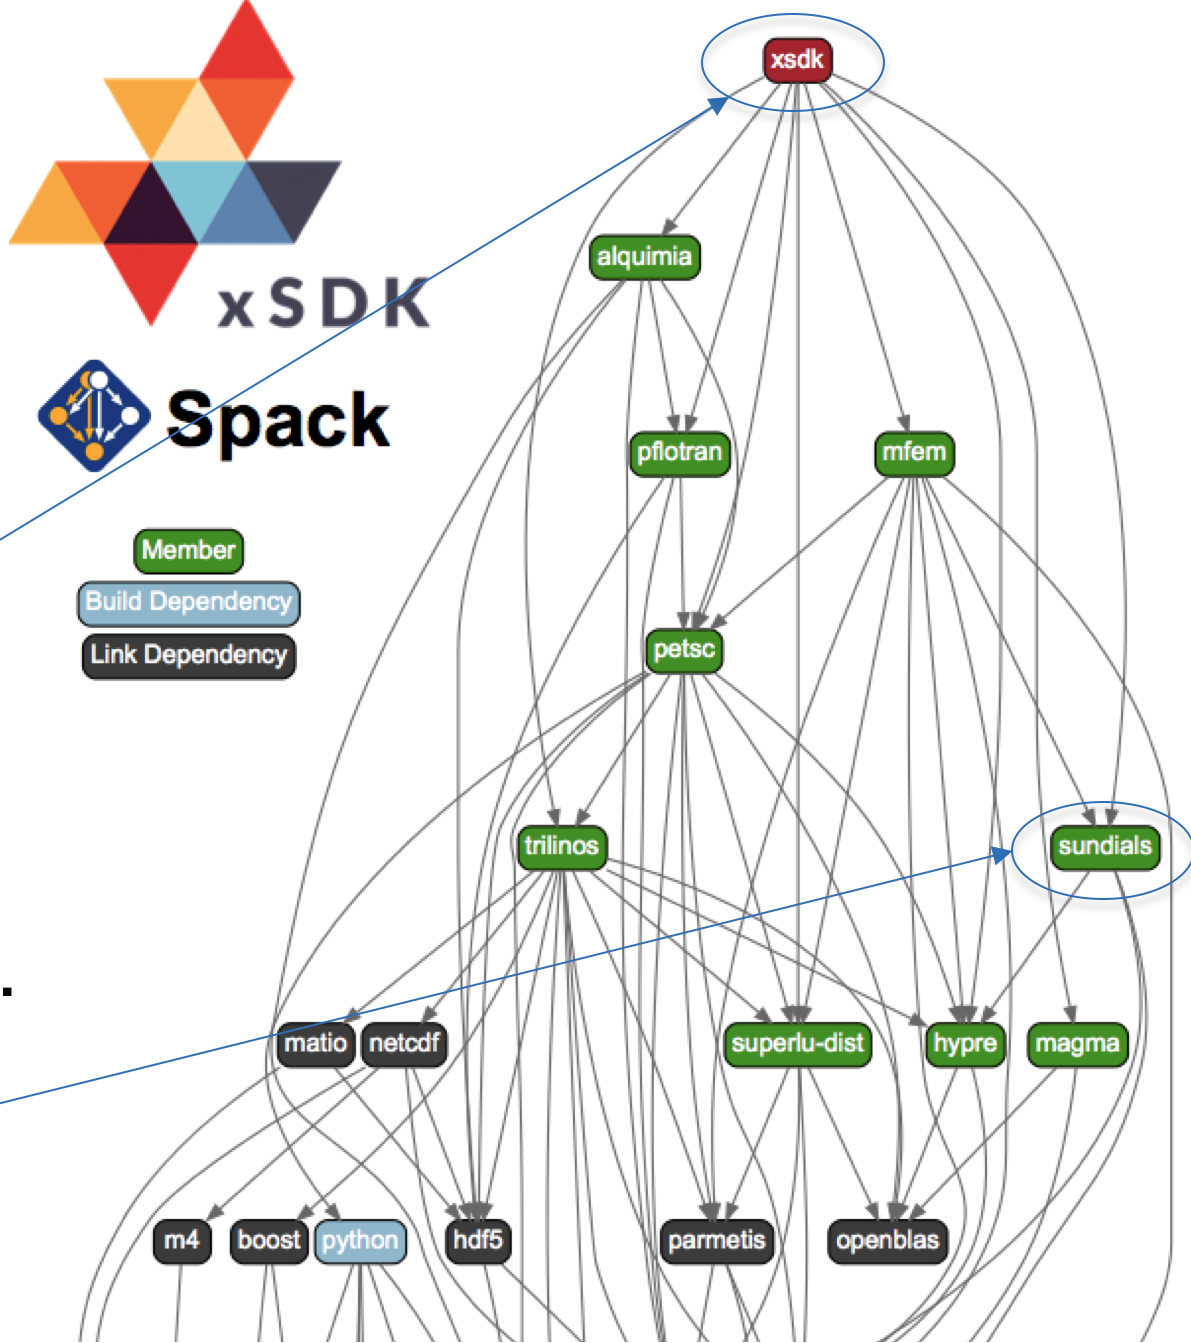
\includegraphics[width=0.9\linewidth]{E4S-Build-Tree}}
	\caption{Using Spack~\cite{gamblin+:ecp18-spack-tutorial}, E4S builds a comprehensive software stack.  As ECP ST efforts proceed, we will use E4S for continuous integration testing, providing developers with rapid feedback on regression errors and providing user facilities with a stable software base as we prepare for Exascale platforms.  This diagram shows how E4S builds ECP products via an SDK target (the math libraries SDK called xSDK in this example).  The SDK target then builds all product that are part of the SDK (see Figure~\ref{fig:sdk-definition1} for SDK groupings), first defining and building external software products. Green-labeled products are part of the SDK. The blue-label indicates expected system tools, in this case a particular version of Python.  Black-labeled products are expected to be previously installed into the environment (a common requirement and easily satisfied).  Using this approach, a user who is interested in only SUNDIALS (a particular math library) can be assured that the SUNDIALS build will be possible since it is a portion of what E4S builds and tests.}
	\label{fig:e4s-build-tree}
\end{figure}

E4S has the following key features:
\begin{itemize}
	\item \textbf{The E4S suite is a large and growing effort to build and test a comprehensive scientific software ecosystem:} E4S V0.1 contained 25 ECP products.  E4S V0.2, release in January 2019 contained 37 ECP products and numerous additional products needed for a complete software environment.  Eventually E4S will contain all open source products to which ECP contributes, and all related products needed for a holistic environment.
	\item \textbf{E4S is not an ECP-specific software suite:}  The products in E4S represent a holistic collection of capabilities that contain the ever-growing SDK collections sponsored by ECP and all additional underlying software required to use ECP ST capabilities.  Furthermore, we expect the E4S effort to live beyond the timespan of ECP, becoming a critical element of the scientific software ecosystem.
	\item \textbf{E4S is partitionable:} E4S products are built and tested together using a tree-based hierarchical build process.  Because we build and test the entire E4S tree, users can build any subtree of interest, without building the whole stack (see Figure~\ref{fig:e4s-build-tree}).
	\item \textbf{E4S uses Spack:} The Spack~\cite{gamblin+:ecp18-spack-tutorial} meta-build tool invokes the native build process of each product, enabling quick integration of new products, including non-ECP products.
	\item \textbf{E4S is available via containers:} In addition to a build-from-source capability using Spack, E4S maintains several container environments (Docker, Singularity, Shifter, CharlieCloud) that provides the lowest barrier to use.  Container distributions dramatically reduce installation costs and provide a ready-made environment for tutorials that leverage E4S capabilities.  For example, the ECP  application project CANDLE (Cancer Deep Learning Environment) uses an E4S container to provide a turnkey tutorial execution environment.
	\item \textbf{E4S distribution:} E4S products are available at \url{http://e4s.io}.
	\item \textbf{E4S developer community resources:} Developers interested in participating in E4S can visit the E4S-Project GitHub community at \url{https://github.com/E4S-Project}.	
\end{itemize}

\begin{figure}
	\centering
	\fbox{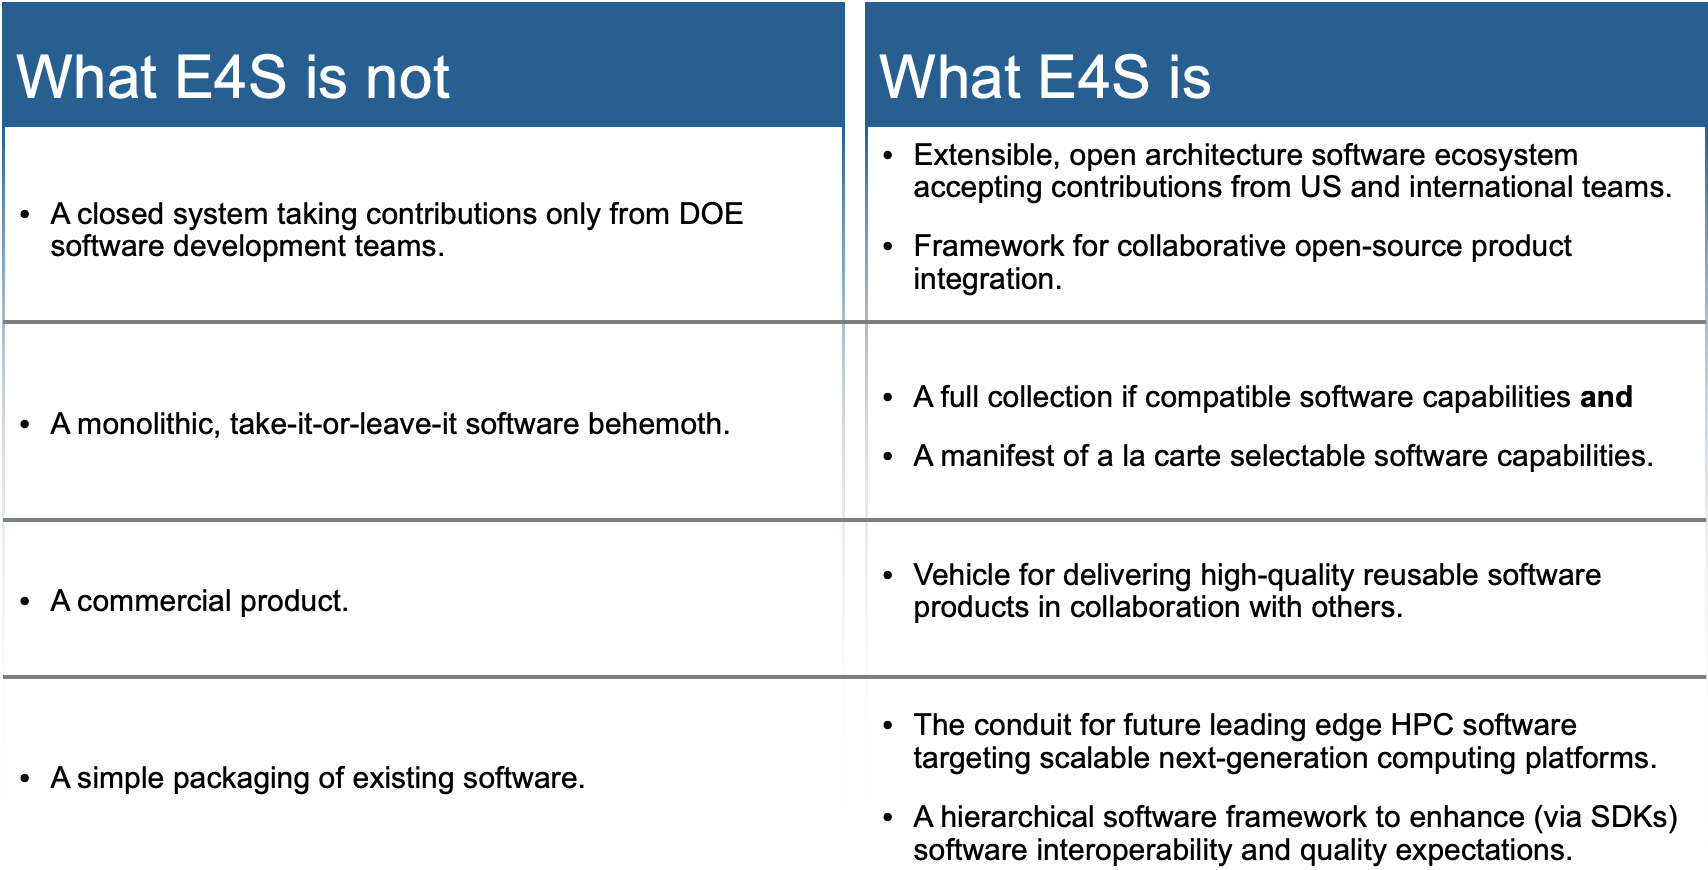
\includegraphics[width=0.9\linewidth]{E4S-Summary}}
	\caption{The Extreme-scale Scientific Software Stack (E4S) provides a complete Linux-based software stack that is suitable for many scientific workloads, tutorial and development environments.  At the same time, it is an open software architecture that can expand to include any additional and compatible Spack-enabled software capabilities. Since Spack packages are available for many products and easily created for others, E4S is practically expandable to include almost any robust Linux-based product.  Furthermore, E4S capabilities are available as subtrees of the full build: E4S is not monolithic.}
	\label{fig:e4s-is-isnot}
\end{figure}

\begin{figure}
	\centering
	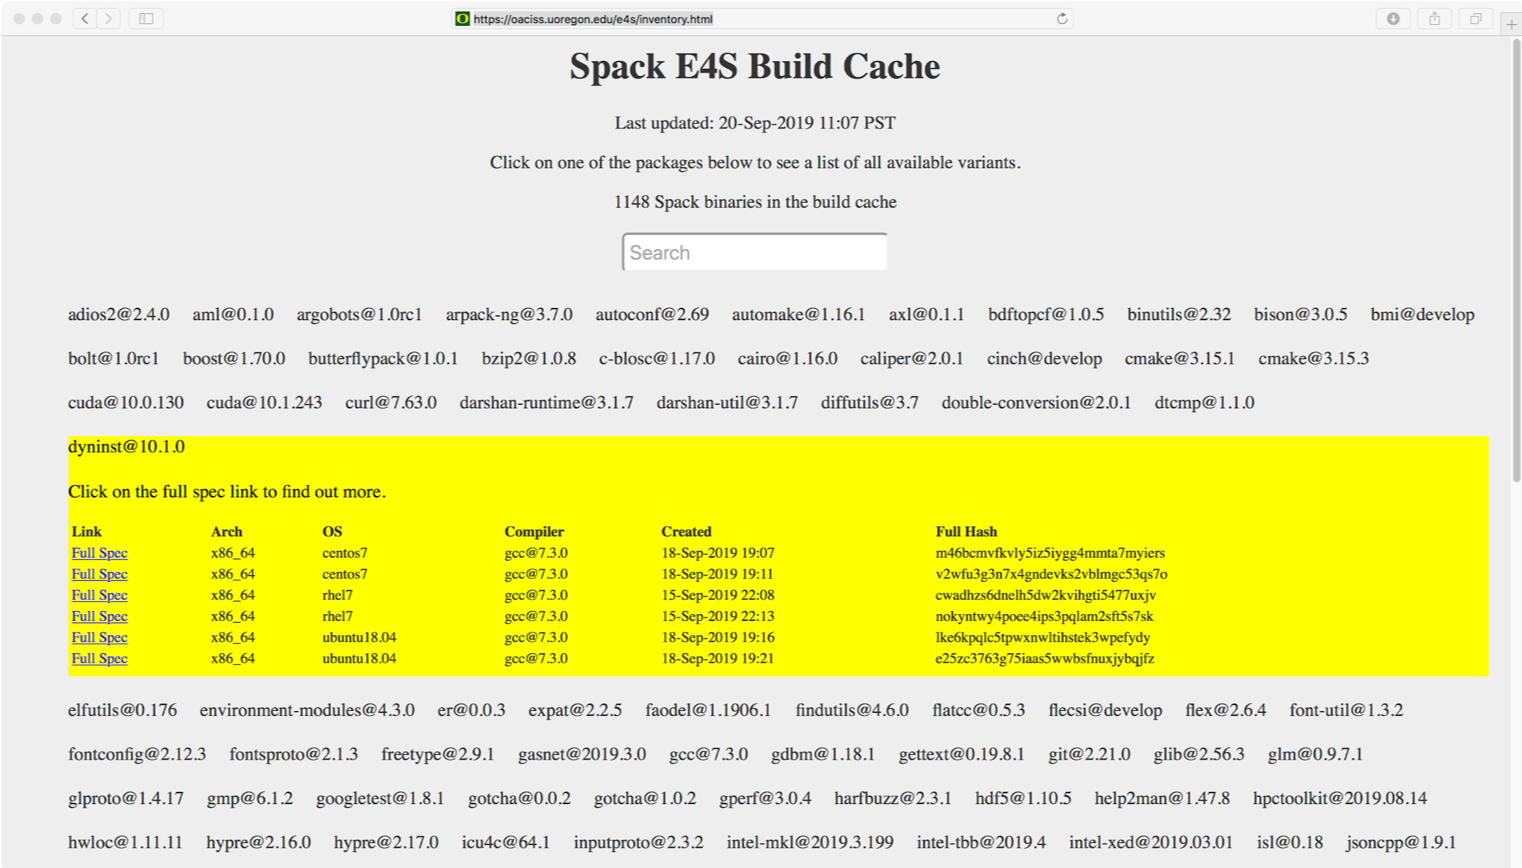
\includegraphics[width=0.9\linewidth]{E4S-Build-Cache-Binaries}
	\caption{Using Spack build cache features, E4S builds can be accelerated by use of cached binaries for any build signature that Spack has already seen.}
	\label{fig:e4s-build-cache}
\end{figure}

\begin{figure}
	\centering
	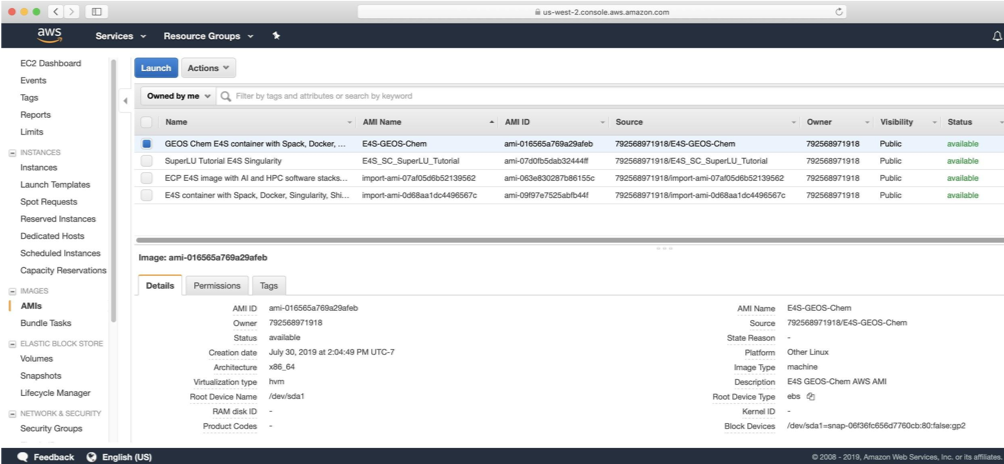
\includegraphics[width=0.9\linewidth]{E4S-AWS-public-image}
	\caption{E4S is available as an Amazon AWS public image.  Images on Google and Microsoft Cloud environments will be available soon.}
	\label{fig:e4s-aws-image}
\end{figure}


The E4S effort is described in further detail in Sections~\ref{subsect:ecosystem}, especially Section~\ref{subsubsect:sdks}.

\subsubsection{Software Development Kits}\label{subsubsect:sdks}
One opportunity for a large software ecosystem project such as ECP ST is to foster increased collaboration, integration and interoperability among its funded efforts. Part of ECP ST design is the creation of software development kits (SDKs).  SDKs are collections of related software products (called packages) where coordination across package teams will improve usability and practices and foster community growth among teams that develop similar and complementary capabilities. SDKs have the following attributes:
\begin{table}
	\begin{mdframed}
\begin{enumerate}
	\item \textbf{Domain scope:} Each SDK will be composed of packages whose capabilities are within a natural functionality domain. Packages within an SDK provide similar capabilities that can enable leveraging of common requirements, design, testing and similar activities. Packages may have a tight complementary such that ready composability is valuable to the user.
	\item \textbf{Interaction models:} How packages within an SDK interact with each other. Interactions include common data infrastructure, or seamless integration of other data infrastructures; access to capabilities from one package for use in another.
	\item \textbf{Community policies:} Expectations for how package teams will conduct activities, the services they provide, software standards they follow, and other practices that can be commonly expected from a package in the SDK.
	\item \textbf{Meta-build system:} Robust tools and processes to build (from source), install and test the SDK with compatible versions of each package. This system sits on top of the existing build, install and test capabilities for each package.
	\item \textbf{Coordinated plans:} Development plans for each package will include efforts to improve SDK capabilities and lead to better integration and interoperability.
	\item \textbf{Community outreach:} Efforts to reach out to the user and client communities will include explicit focus on SDK as product suite.
\end{enumerate}
	\end{mdframed}
\caption{\label{table:sdk-attributes} Software Development Kits (SDKs) provide an aggregation of software products that have complementary or similar attributes.  ECP ST uses SDKs to better assure product interoperability and compatibility.  SDKs are also essential aggregation points for coordinated planning and testing. SDKs are an integral element of ECP ST~\cite{Heroux-SDK-Podcast}.  Section~\ref{subsubsect:ecosystem-sdk} describes the six SDK groupings and the current status of the SDK effort.}
\end{table}

\paragraph{ECP ST SDKs}
As part of the delivery of ECP ST capabilities, we will establish and grow a collection of SDKs. The new layer of aggregation that SDKs represent are important for improving all aspects of product development and delivery. The communities that will emerge from SDK efforts will lead to better collaboration and higher quality products. Established community policies will provide a means to grow SDKs beyond ECP to include any relevant external effort. The meta-build systems (based on Spack) will play an important role in managing the complexity of building the ECP ST software stack, by providing a new layer where versioning, consistency and build options management can be addressed at a mid-scope, below the global build of ECP ST products.
Each ECP ST L3 (five of them) has funds for an SDK project from which we have identified a total of six SDKs and an at-large collection of remaining products that will be delivered outside of the SDK grouping.  Section~\ref{subsubsect:ecosystem-sdk} provides an update on the progress in defining SDK groupings. For visibility, we provide the same diagram in Figure~\ref{fig:sdk-definition1-0}.

\begin{figure}[htb]
	\centering
	\fbox{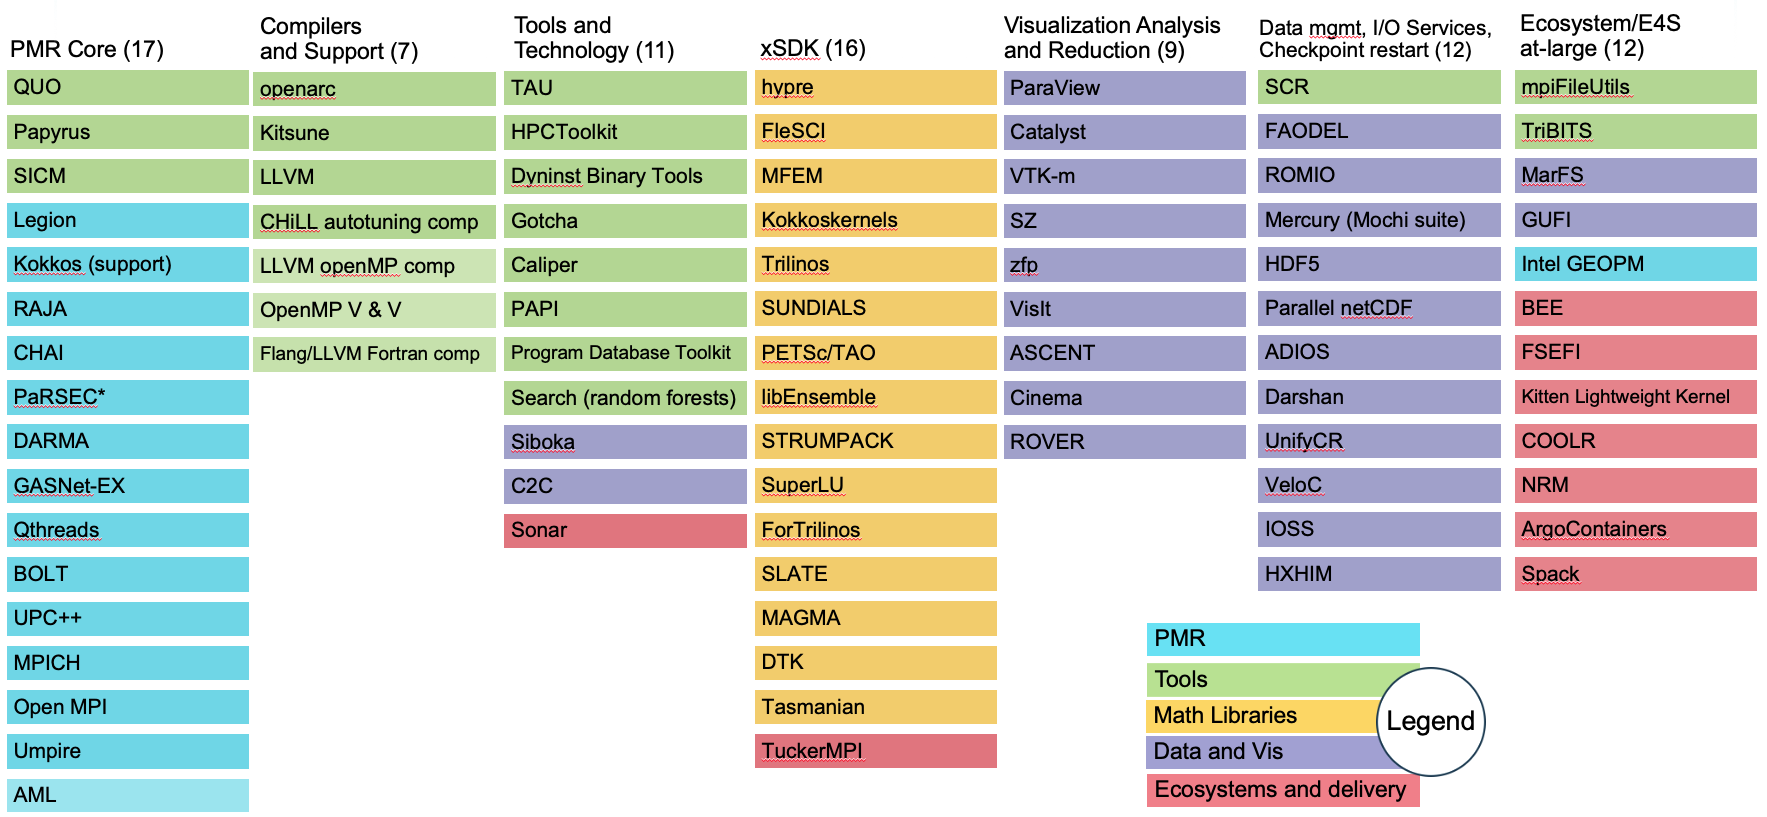
\includegraphics[width=6.5in]{projects/2.3.5-Ecosystem/2.3.5.01-Ecosystem-SDK/SDKdefinition2}}
	\caption{\label{fig:sdk-definition1-0}The above graphic shows the breakdown of ECP ST products into 6 SDKs ( the first six columns).  The rightmost column lists products that are not part of an SDK, but are part of Ecosystem group that will also be delivered as part of E4S. The colors denoted in the key map all of the ST products to the ST technical area they are part of.  For example, the xSDK consists of products that are in the Math Libraries Technical area, plus TuckerMPI which is in the Ecosystem and Delivery technical area.  Section~\ref{subsubsect:ecosystem-sdk} provides an update on the progress in defining SDK groupings.}
\end{figure}


\subsubsection{ECP ST Product Dictionary}\label{subsubsect:dictionary}
In the past year, ECP has initiated an effort to explicitly manage ECP ST products and their dependencies (see Section~\ref{subsubsect:dep-management}).  In order to eliminate ambiguities, we first need a product dictionary: an official list of publicly-name products to which ECP ST teams contribute their capabilities and upon which ECP ST clients depend.  The ECP Product Dictionary is single, managed table.  It presently contains 70 primary products along with subproducts that are either components within a product or particular implementations if a standard API.  Two special primary products are the Facilities stack and Vendor stack.  Having these stacks on the list enables ST teams to indicate that their capabilities are being delivered to ecosystems outside of ECP.

Figure~\ref{fig:product-dictionary-overview} describes the policy for ECP ST teams to add and manage their contributions to the Product Dictionary.  Figure~\ref{fig:product-dictionary} shows a snapshot of the beginning and end of the current ECP ST Product Dictionary, which is maintained on the ECP Confluence wiki.

\begin{figure}
	\centering
	\fbox{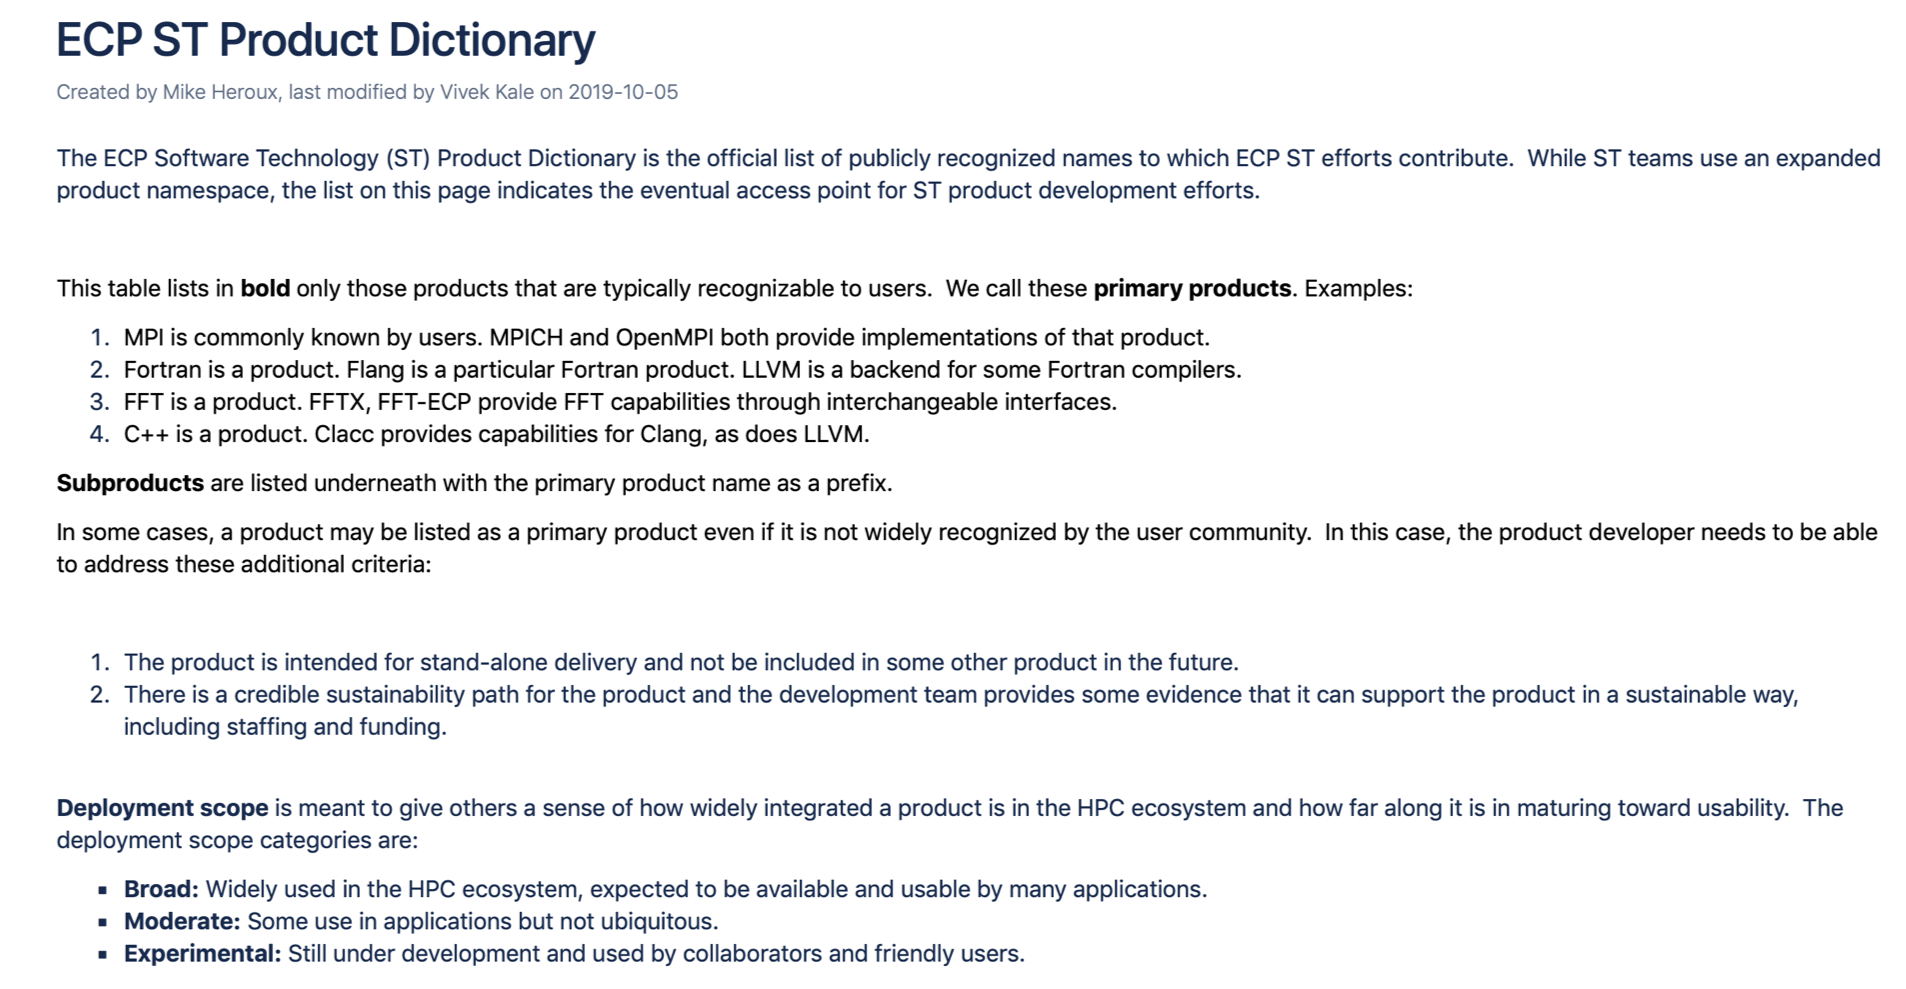
\includegraphics[width=0.9\linewidth]{ProductDictionaryOverview}}
	\caption{This figure shows a screenshot from the top of the ECP Confluence wiki page containing the ECP ST Product Dictionary.  The Product Dictionary structure contains primary and secondary products.  Client (consumer) dependencies are stated against the primary product names only, enabling unambiguous mapping of AD-on-ST and ST-on-ST dependencies.}
	\label{fig:product-dictionary-overview}
\end{figure}

\begin{figure}
	\centering
	\fbox{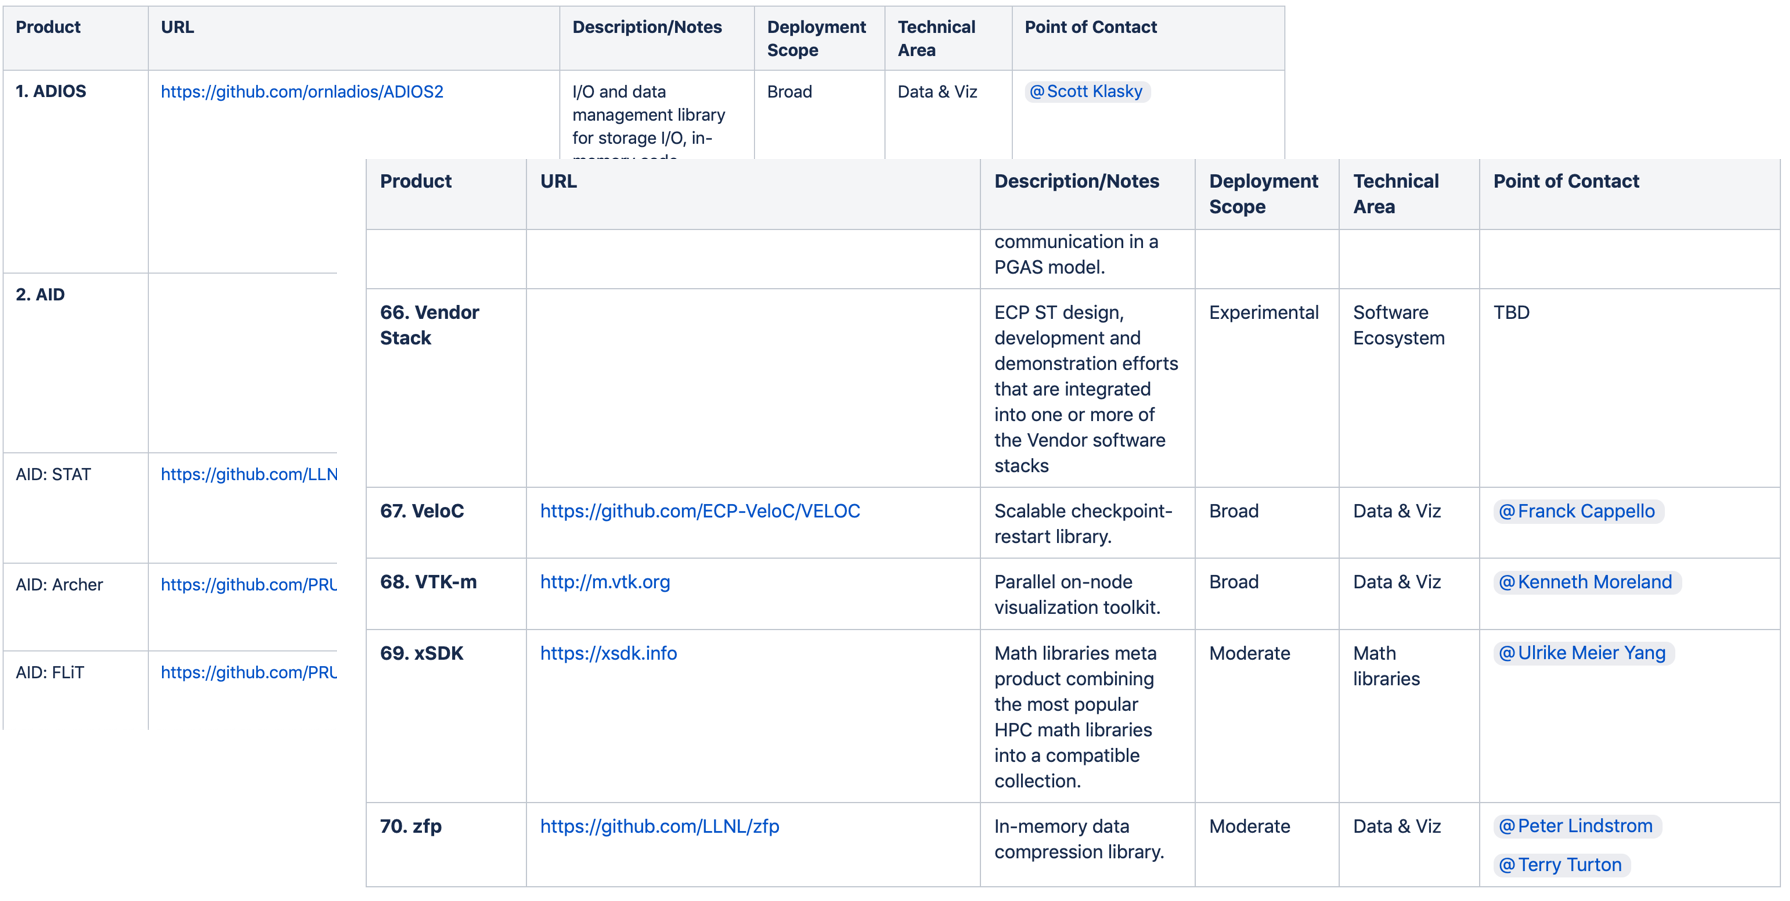
\includegraphics[width=0.9\linewidth]{ConfluenceProductDictionaryExample}}
	\caption{These screen shots are from the ECP Confluence Product Dictionary Table.  The table is actively managed to include primary and secondary products to which ECP ST team contribute and upon which ECP ST clients depend.  Presently the Product Dictionary contains 70 primary products.  Secondary products are listed under the primary product with the primary product as a prefix.  For example, AID is the second listed primary product in this figure.  STAT, Archer and FLIT are component subproducts.  MPI (not shown) is another primary product.  MPICH and OpenMPI are two robust MPI implementations and are listed as MPI subproducts.}
	\label{fig:product-dictionary}
\end{figure}

\subsubsection{ECP Product Dependency Management}\label{subsubsect:dep-management}
Given the ECP ST Product Dictionary, and a similar dictionary for ECP AD and Co-Design products, ECP as a project has created a dependency database that enabled creation and characterization of product-to-product dependencies.  ECP manages these dependencies in a Jira database using a custom Jira issue type, Dependency.  The dependency database provides an important tool for understanding and managing ECP activities.  The dependency information is valuable both within and outside the project.  Figure

\begin{figure}
	\centering
	\fbox{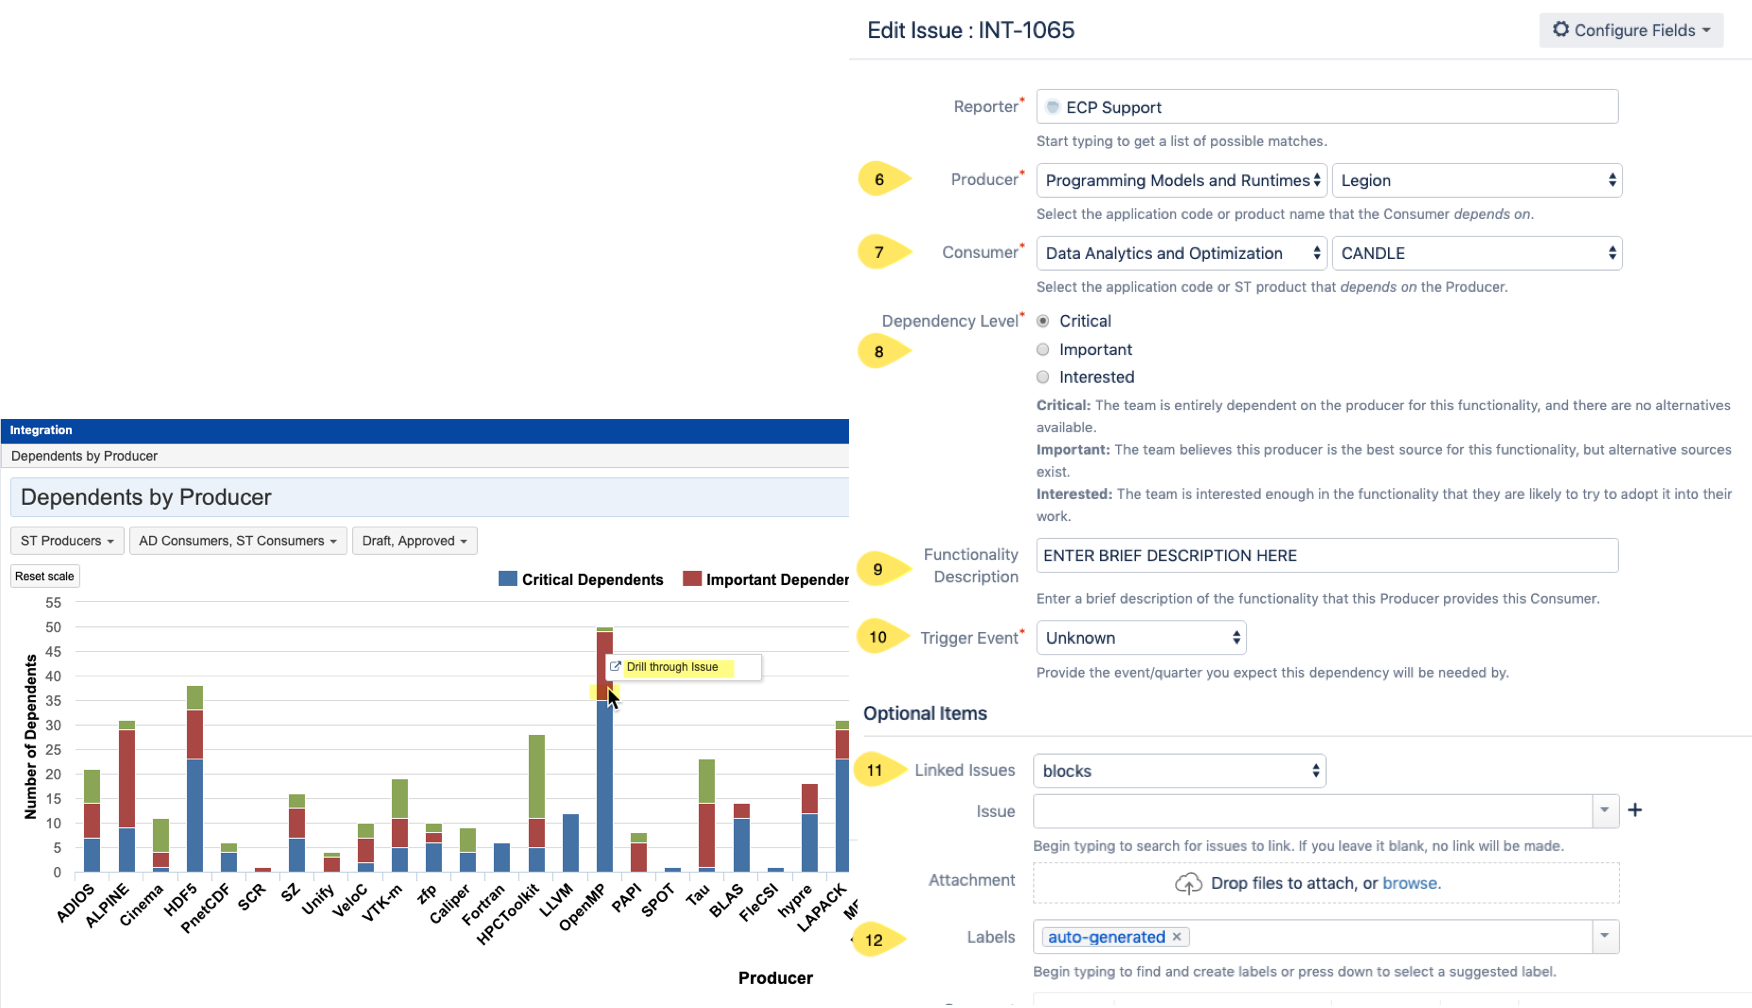
\includegraphics[width=0.9\linewidth]{DependencyDashboard-EditPanel}}
	\caption{Using Jira, ECP manages its AD, ST, HI, vendor and facilities dependencies.  This figure shows a dashboard snapshot along with an edit panel that support creation and management of a consumer-on-producer dependency.}
	\label{fig:dependency-dashboard-edit}
\end{figure}

\begin{figure}
	\centering
	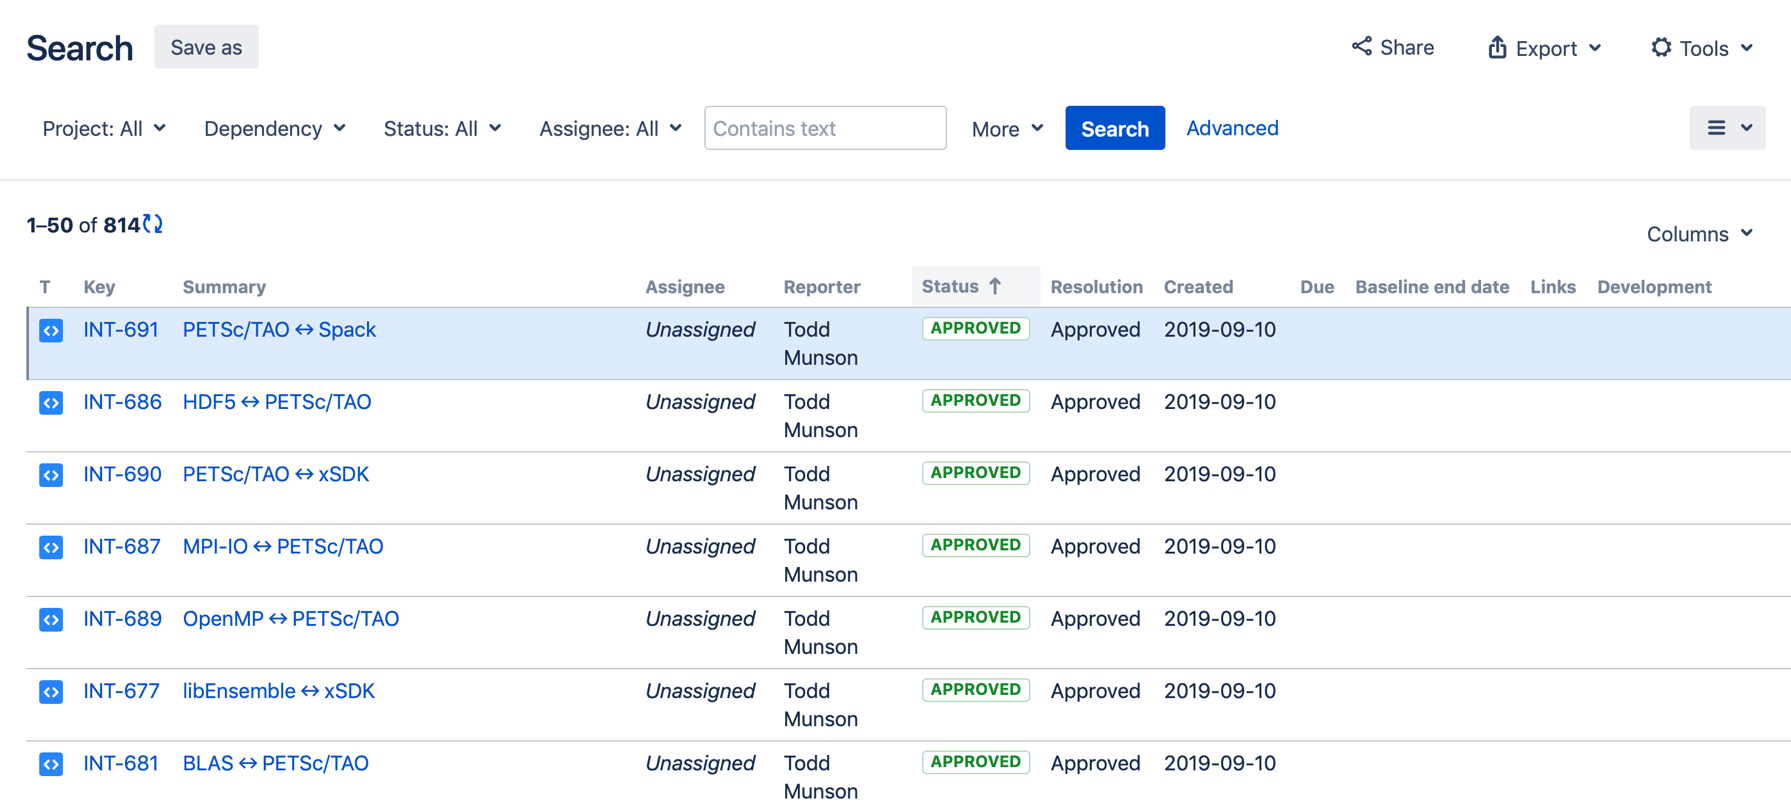
\includegraphics[width=0.9\linewidth]{PETSc-TAO-Dependencies}
	\caption{This query result from the ECP Jira Dependency database lists all consumers of capabilities from the PETSc/TAO product.  By selecting the details of one of the dependency issues, one can further see how critical the dependency is and see any custom information peculiar to the particular dependency.}
	\label{fig:petsc-tao-dependencies}
\end{figure}

\newpage
\subsection{ECP ST Planning and Tracking}

While ECP is an official 413.3b federal construction project using an earned value management (EVM) structure, we are permitted to tailor the planning process in order to obtain the flexibility needed for a software project whose requirements are emerging as the project proceeds.  In this section, we describe how ECP ST plans it activities using the Jira project management tool.  We first discuss P6 Activities (similar to milestones) and then discuss the key performance parameter (KPP-3) associated with ECP ST.


\subsubsection{ECP ST P6 Activity Issues}

ECP ST uses a custom Jira issue type called P6 Activity.  Each L4 subproject creates a series of P6 Activity issues extending to the end of ECP (Q3FY23).  Except for the current fiscal year, a single P6 Activity issue describes expected deliverables as a planning package.  Six months prior to the start of a fiscal year, the planning package for the coming year is replaced with 4--6 issues spanning the year with baseline start and end dates, an estimate of the percent annual budget and a high level description.  Eight weeks prior to the start of an activity, full details about staffing, completion criteria and more are added to the issue.  Figure~\ref{fig:planning-process} show the steps in diagram form.  

Cost, scope and schedule for ECP ST is tracked and managed by monitoring progress of the collection of P6 Activities.  Value is accrued when a P6 Activity issue is marked Done in the Jira database.  Schedule and cost performance indices are derived from the status of our P6 Activities.  Schedule, cost and scope changes against the plan are managed via a formal project change request (PCR) process.

\begin{figure}
	\centering
	\fbox{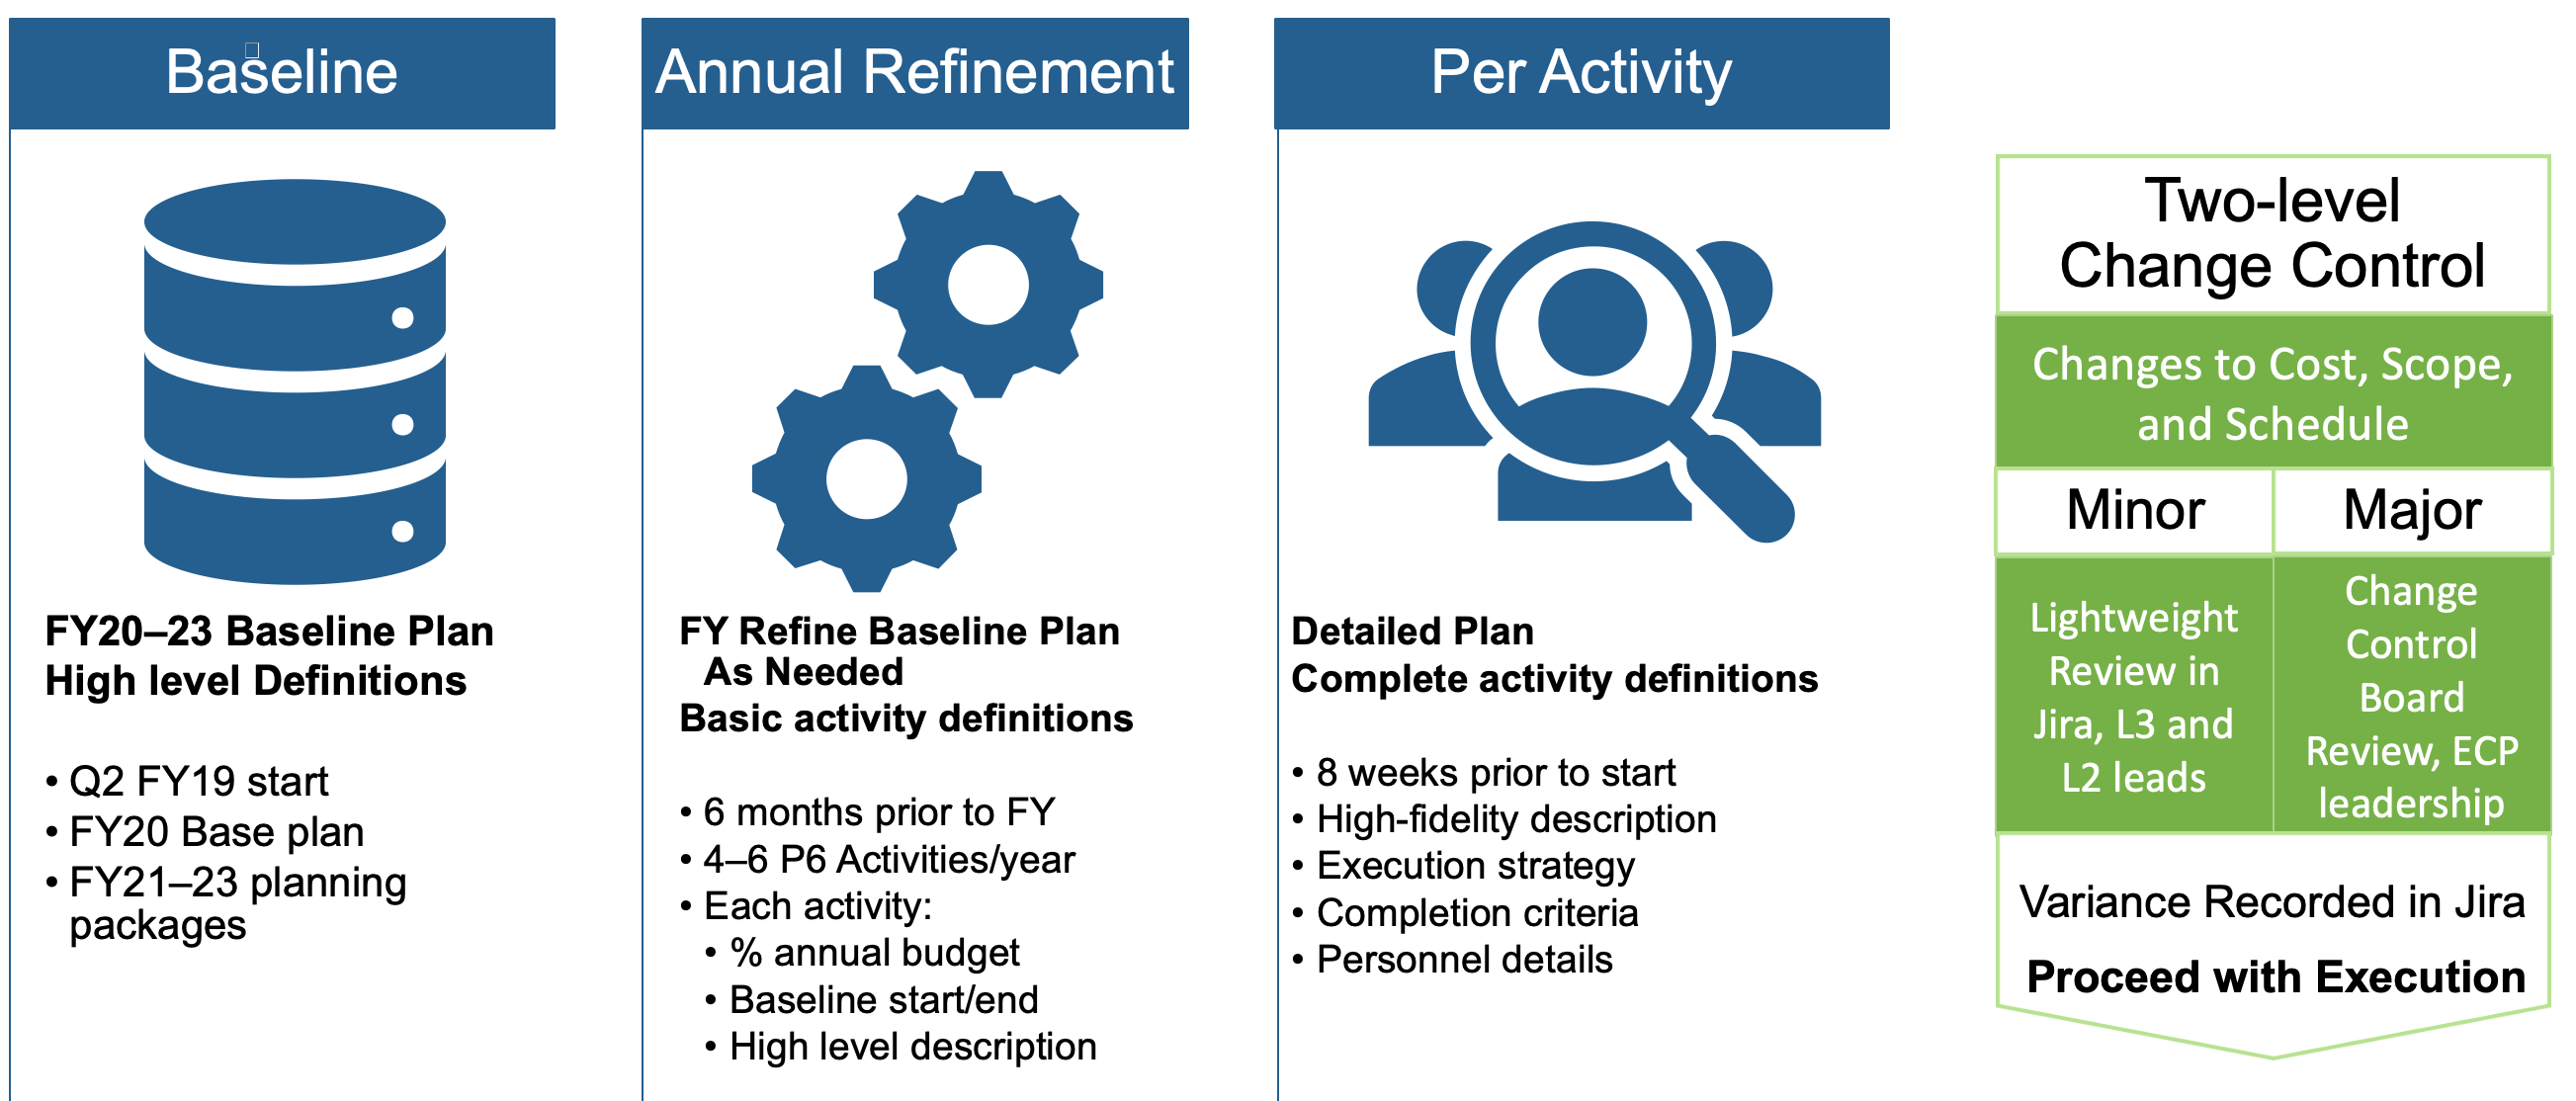
\includegraphics[width=0.9\linewidth]{Planning-Process}}
	\caption{ECP ST uses a custom Jira issue type called P6 Activity.  Each L4 subproject creates a series of these issues extending to the end of ECP.  Except for the current fiscal year, a single P6 Activity issue describes expected deliverables as a planning package.  Six months prior to the start of a fiscal year, the planning package is replaced with 4--6 issues spanning the coming year.  Eight weeks prior to the start of an activity, full details about staffing, completion criteria and more are added to the issue.}
	\label{fig:planning-process}
\end{figure}


\subsubsection{Key Performance Parameter (KPP) 3}

ECP has four Key Performance Parameters (KPPs).  Figure~\ref{fig:kpp-definitions} shows the KPP definitions. KPP-3 is focused on a productive and sustainable software ecosystem. ECP ST is the primary owner of this KPP (along with co-design projects in ECP AD).  The focus of KPP-3 is defining and tracking capability integrations of ST products into client environment, as described in this section. 

\begin{figure}
	\centering
	\fbox{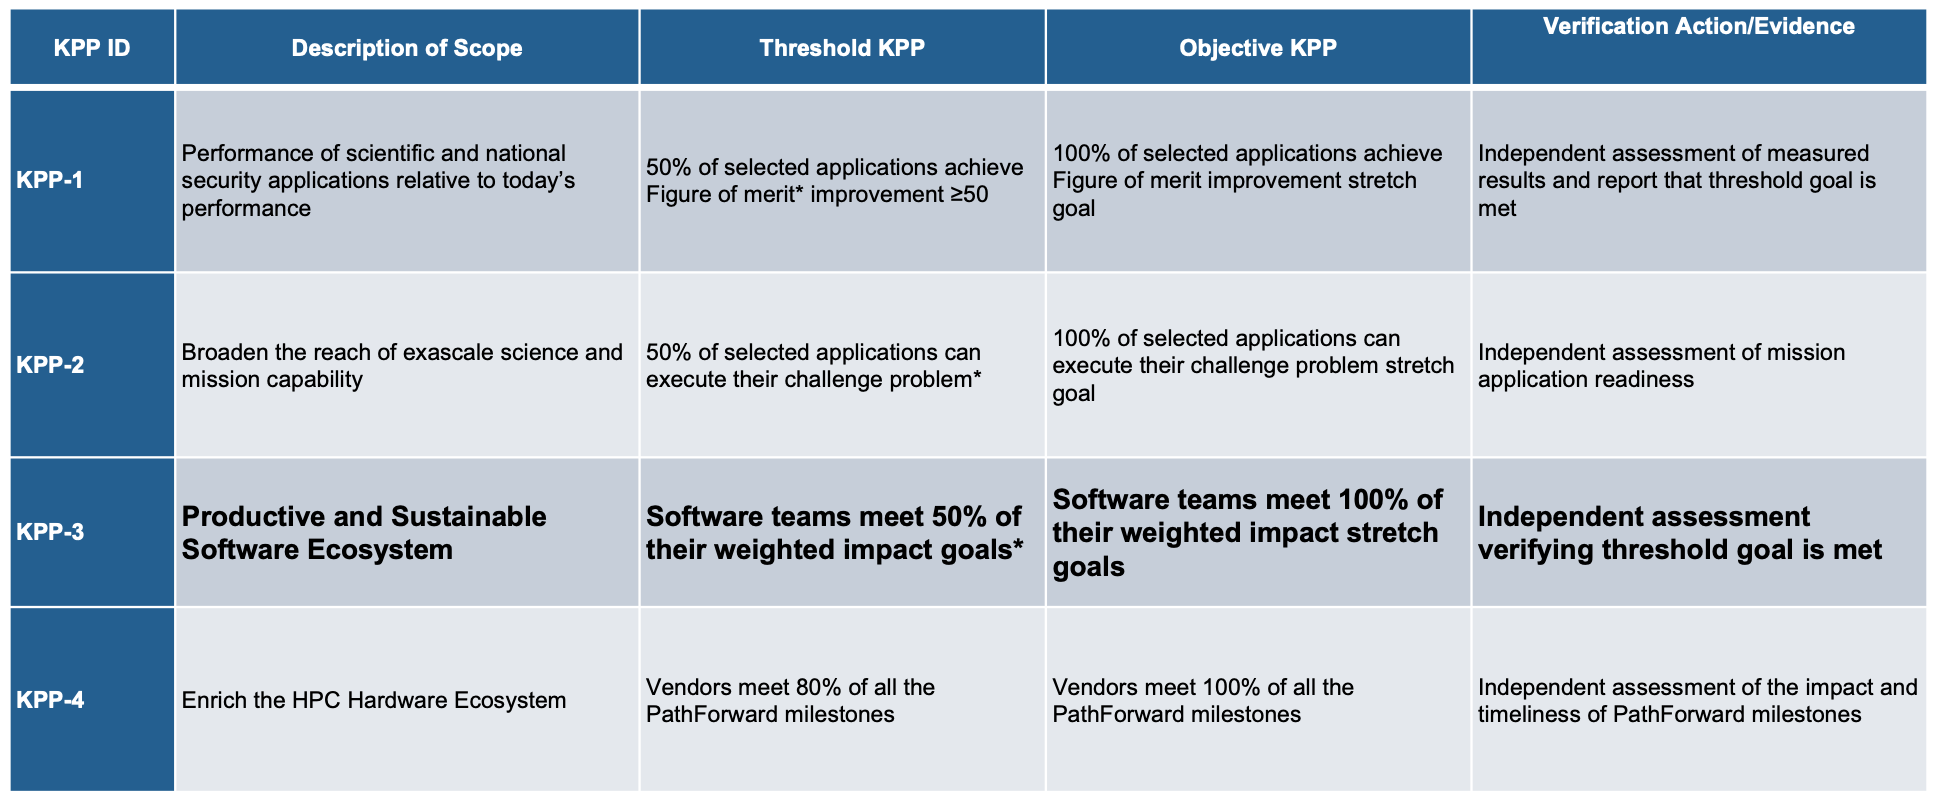
\includegraphics[width=0.9\linewidth]{KPP-Definitions}}
	\caption{ECP has four key performance parameters (KPPs).  ECP ST is the primary owner (with ECP AD co-design subprojects) of KPP-3.}
	\label{fig:kpp-definitions}
\end{figure}



First, we define terms:
\begin{itemize}
	\item \textbf{Capability:} Any significant product functionality, including existing features adapted to the pre-exascale and exascale environments, that can be integrated into a client environment.
	\item \textbf{Integration Goal:} A statement of impact on the ECP ecosystem where a software capability is used in a consequential and sustainable way by a client in pre-exascale environments first, then in exascale environments.  Integration goals are product focused.  A project that contributes to more than one product will have a KPP-3 Jira issue for each of its products.
	\item \textbf{Integration Score: }The number of successful capability integrations into a client environment.
	\item \textbf{Sustainable:} For the purposes of KPP-3, sustainable means that the capability is integrated in a way that reasonably assures future use of the capability beyond the end of ECP.  For libraries, this would generally mean that library usage is made from source code in the main repository and use of the library is tested regularly as a part of the client code regular regression testing.  For tools, sustainable would generally mean the tool is available as needed in the exascale environment.  For prototype capabilities that are incorporated into vendor and community software, the impact of the prototype is still visible to a subject matter expert.
\end{itemize}

\paragraph{Defining an Integration Goal}
Integration goals are defined per product within each project.  The goal statement will include:
\begin{itemize}
	\item The name of the product to which the project contributes.  The product must be listed in the ECP ST Product Dictionary.
	\item A description of the target clients into whose environments the product capabilities will be integrated.  Specific clients can be listed, but are not necessary.  Clients must be part of ECP, or otherwise part of the exascale systems ecosystem such as a vendor or facility partner.   
	\item A general description of the nature of the integration, addressing what it means to be successfully integrated.
\end{itemize}

\begin{table}[h!]
	\begin{tabular}{|L{1.5in}|L{2.0in}|L{2.5in}|}\hline
		\rowcolor{LightCyan}
		Integration Score & Capability & Integration Description\\\hline
		1 point per capability sustainably integrated by a client, per exascale platform used. &
		Complete, sustainable integration of a significant product capability into a client environment in a pre-exascale environment (tentative score) and in an exascale environment (confirmed score). &
		Client acknowledges benefit from product capability use and considers it part of their workflow. Integration is sustainable with documentation and testing. Integration of product capability into main product repo and SDK/E4S environments is completed.\\\hline
	\end{tabular}
	\caption{\label{table:KPP-3-scoring} Integration Goal Scoring: A point is accrued when a client integrates and sustainably uses a product's capabilities.  Scores are assessed annually.}
\end{table}


\paragraph{Demonstration and recording of progress toward integration goal}
All artifacts and evidence of progress will be captured in the Jira KPP-3 issue associated with a product integration goal as progress is made.  All integration scores are tentative until the capability is available and demonstrated in exascale environments.  Table~\ref{table:KPP-3-values} summarizes the defined values.

\begin{table}[h!]
	\begin{tabular}{|L{0.6in}|L{2.0in}|L{3.4in}|}\hline
		\rowcolor{LightCyan}
		Value & Definition & Description\\\hline
		Present & The current integration score. & This is always an indication of the progress the team has made. The present value is assessed annually.\\\hline
		Passing & The minimum integration score required for the product to be counted as part of ECP ST progress toward KPP-3. & The passing score is between 4 and 8 for each integration goal, 4 for larger integration efforts, 8 for smaller ones. This is equivalent to accomplishing one to two capability integration per year per product.\\\hline
		Stretch & The maximum reasonably achievable integration score for a product if capability integrations are successful with all potential ECP clients.   & The stretch value allows us to see the overall integration potential.\\\hline
	\end{tabular}
	\caption{\label{table:KPP-3-values} Key metric values: These values are determined by the L4 sub-project team when defining their KPP-3 issue.}
\end{table}

\paragraph{Assessment process}
While progress is recorded as it is achieved, progress assessment is done annually, including input from external subject matter experts (SMEs).  ECP leadership and SMEs will review integration score evidence, confirming or adjusting integration scores.
Note: Assessment can result in a reduced integration score from a previous year if a client has stopped using a capability that was previously used.

\paragraph{Transition from tentative to confirmed integration score}
Each integration score is tentative until the capability is available and demonstrated to be effective in the exascale environments.  Demonstration can be achieved by a variety of means such that ECP Leadership and SMEs are reasonably certain the capability positively impacts the client in exascale environments.  At this point the integration score becomes confirmed. 
Typically, the transition from tentative to confirmed would be a low-cost independent demonstration, or accomplished within the client’s environment as the client is conducting its own assessments. 
Note: The planned exascale system (El Capitan) that can support National Security applications will not be available until the end of FY23. Integration of ST products into National Security Applications will be considered for transition from tentative to confirmed when either a) evidence of integration is provided during FY20-22 ASC L1 and L2 milestones related to ECP/ATDM National Security application readiness for exascale platforms, and/or b) integration is demonstrated on the El Capitan early access systems, and exercises capabilities similar to those anticipated to be important to effectively using El Capitan.  For KPP-3 capability integrations targeted at El Capitan, we will use the best available confirmation process in FY23.
KPP-3 weighted scoring

\begin{table}[h!]
	\begin{tabular}{|L{1.0in}|L{0.5in}|L{4.5in}|}\hline
		\rowcolor{LightCyan}
		Impact Level & Weight & Comments\\\hline
		High & 2 & The score for integration goals associated with high impact products will be added to the KPP-3 score with a weight of 2.\\\hline
		Normal & 1 & Most KPP-3 Jira issues will have a weight of one.\\\hline
		Risk-Mitigating & 0.5 & Some KPP-3 Jira issues are associated with products that help us plan for the potential risks if high impact products don’t deliver as expected.\\\hline
		Shared  & 0.5 & Some projects receive funding from both NNSA and SC, e.g. RAJA/Kokkos. For these projects, the score is balanced to reflect dual contributions.\\\hline
	\end{tabular}
	\caption{\label{table:KPP-3-impact} Each integration score will have an associated weight depending on the potential impact if integration targets are not met.}
\end{table}

The KPP-3 score is the weighted sum of all integration goals that have an integration score that meets or exceeds its passing value. 
The KPP-3 score will initially be tentative.  The KPP-3 score is not officially met until the weighted sum of confirmed integration scores exceeds 50% of the total possible points.


\subsubsection{ECP ST Software Delivery}
An essential activity for, and the ultimate purpose of, ECP ST is the delivery of a software stack that enables productive and sustainable Exascale computing capabilities for target ECP applications and platforms, and the broader high-performance computing community. The ECP ST Software Ecosystem and Delivery sub-element (WBS 2.3.5) and the SDKs in each other sub-element provide the means by which ECP ST will deliver its capabilities.
\paragraph{ECP ST Delivery and HI Deployment}
Providing the ECP ST software stack to ECP applications requires coordination between ECP ST and ECP HI. The focus areas have a complementary arrangement where ECP ST delivers its products and ECP HI deploys them. Specifically:
\begin{itemize}
	\item ST \textbf{delivers} software.  ECP ST products are delivered directly to application teams, to vendors and to facilities.  ECP ST designs and implements products to run on DOE computing facilities platforms and make products available as source code via GitHub, GitLab or some other accessible repository.
	\item HI facilitates efforts to \textbf{deploy} ST (and other) software on Facilities platforms by installing it where users expect to find it. This could be in /usr/local/bin or similar directory, or available via “module load”.
\end{itemize}
Separating the concerns of delivery and deployment is essential because these activities require different skill sets. Furthermore, ECP ST delivers its capabilities to an audience that is beyond the scope of specific Facilities’ platforms. This broad scope is essential for the sustainability of ECP ST products, expanding the user and developer communities needed for vitality. In addition, ECP HI, the computer system vendors and other parties provide deployable software outside the scope of ECP ST, therefore having the critical mass of skills to deploy the entire software stack.

\paragraph{ECP ST Delivery Strategy}
ECP ST delivers it software products as source code, primarily in repositories found on GitHub, Gitlab installations or similar platforms. Clients such as ECP HI, OpenHPC and application developers with direct repository access then take the source and build, install and test our software. The delivery strategy is outlined in Figure~\ref{fig:softwarestack}.  

Users access ECP ST products using these basic mechanisms:
\begin{itemize}
	\item \textbf{Build from source code:} The vast majority of ECP ST products reach at least some of their user base via direct source code download from the product repository.  In some cases, the user will download a single compressed file containing product source, then expand the file to expose the collection of source and build files.  Increasingly, users will fork a new copy of an online repository.  After obtaining the source, the user executes a configuration process that detects local compilers and libraries and then builds the product.  This kind of access can represent a barrier for some users, since the user needs to build the product and can encounter a variety of challenges in that process, such as an incompatible compiler or a missing third-party library that must first be installed.  However, building from source can be a preferred approach for users who want control over compiler settings, or want to adapt how the product is used, for example, turning on or off optional features, or creating adaptations that extend product capabilities.  For example, large library frameworks such as PETSc and Trilinos have many tunable features that can benefit from the user building from source code.  Furthermore, these frameworks support user-defined functional extensions that are easier to support when the user builds the product from source.  ECP ST is leveraging and contributing to the development of Spack~\cite{gamblin+:sc15}.  Via meta-data stored in a Spack \textit{package} defined for each product, Spack leverages a product's native build environment, along with knowledge about its dependencies, to build the product and dependencies from source.  Spack plays a central role in ECP ST software development and delivery processes by supporting turnkey builds of the ECP ST software stack for the purposes of continuous integration testing, installation and seamless multi-product builds.
	\item \textbf{DOE computing facilities:} Each DOE computing facility (ALCF, OLCF, NERSC, LLNL and ACES [LANL/SNL]) provides pre-built versions of 17 to 20 ECP ST products (although the exact mix of products varies somewhat at each site).  Many of these products are what users would consider to be part of the core system capabilities, including compilers, e.g., Flang (Section~\ref{subsubsect:flang}) and LLVM (Section~\ref{subsubsect:sollve}), and parallel programming environments such as MPICH (Section~\ref{subsubsect:mpich}), OpenMPI (Section~\ref{subsubsect:openmpi}) and OpenMP (Section~\ref{subsubsect:bolt}).  Development tools such as PAPI (Section~\ref{subsubsect:exapapi}) and TAU (Section~\ref{subsubsect:tau}) are often part of this suite, if not already included in the vendor stack. Math and data libraries such as PETSc (Section~\ref{subsubsect:petsc}), Trilinos (Section~\ref{subsubsect:peeks}), HDF5 (Section~\ref{subsubsect:exahdf5}) and others are also available in some facilities software installations.  We anticipate and hope for increased collaboration with facilities via the ECP Hardware \& Integration (HI) Focus Area.  We are also encouraged by multi-lab efforts such as the Tri-Lab Operating System Stack (TOSS)~\cite{TOSS} that are focused on improving uniformity of software stacks across facilities.
	\item \textbf{Vendor stacks:} Computer system vendors leverage DOE investments in compilers, tools and libraries.  Of particular note are the wide use of MPICH(Section~\ref{subsubsect:mpich}) as software base for most HPC vendor MPI implementations and the requirements, analysis, design and prototyping that ECP ST teams provide.  Section~\ref{subsection:external-contributions} describes some of these efforts.
	\item \textbf{Binary distributions:} Approximately 10 ECP ST products are available via binary distributions such as common Linux distributions, in particular via OpenHPC\cite{OpenHPC}.  ECP ST intends to foster growth of availability via binary distributions as an important way to increase the size of the user community and improve product sustainability via this broader user base.
\end{itemize}

\begin{figure}
	\centering
	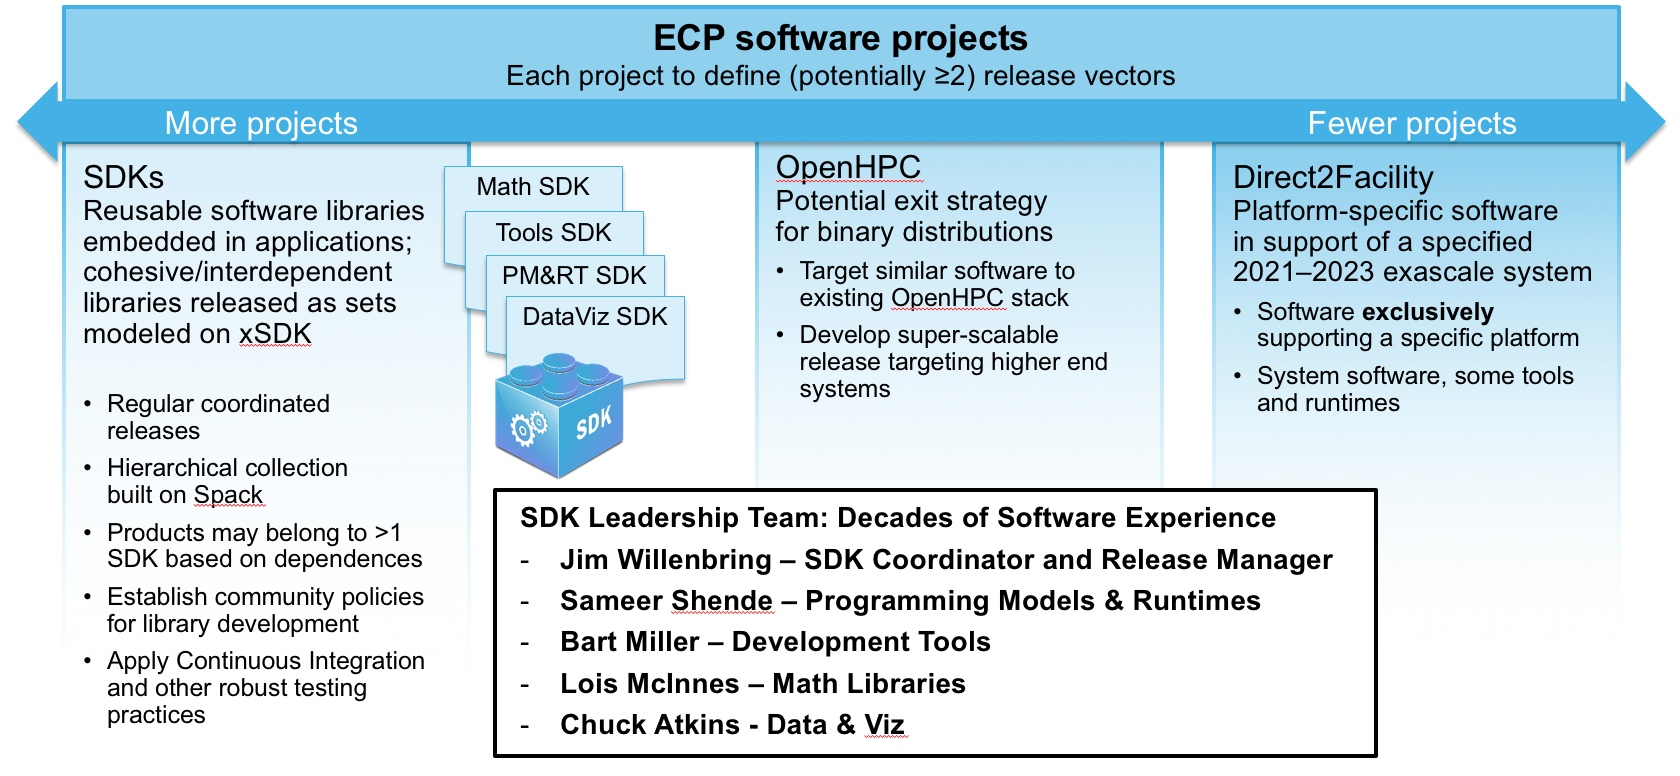
\includegraphics[width=0.9\linewidth]{SoftwareStack}
	\caption{\textbf{The ECP ST software stack is delivered to the user community through several channels.} Key channels are via source code, increasingly using SDKs, direct to Facilities in collaboration with ECP HI, via binary distributions, in particular the OpenHPC project and via HPC vendors.  The SDK leadership team includes  ECP ST team members with decades of experience delivering scientific software products.}
	\label{fig:softwarestack}
\end{figure}

